
%% bare_conf.tex
%% V1.4b
%% 2015/08/26
%% by Michael Shell
%% See:
%% http://www.michaelshell.org/
%% for current contact information.
%%
%% This is a skeleton file demonstrating the use of IEEEtran.cls
%% (requires IEEEtran.cls version 1.8b or later) with an IEEE
%% conference paper.
%%
%% Support sites:
%% http://www.michaelshell.org/tex/ieeetran/
%% http://www.ctan.org/pkg/ieeetran
%% and
%% http://www.ieee.org/

%%*************************************************************************
%% Legal Notice:
%% This code is offered as-is without any warranty either expressed or
%% implied; without even the implied warranty of MERCHANTABILITY or
%% FITNESS FOR A PARTICULAR PURPOSE! 
%% User assumes all risk.
%% In no event shall the IEEE or any contributor to this code be liable for
%% any damages or losses, including, but not limited to, incidental,
%% consequential, or any other damages, resulting from the use or misuse
%% of any information contained here.
%%
%% All comments are the opinions of their respective authors and are not
%% necessarily endorsed by the IEEE.
%%
%% This work is distributed under the LaTeX Project Public License (LPPL)
%% ( http://www.latex-project.org/ ) version 1.3, and may be freely used,
%% distributed and modified. A copy of the LPPL, version 1.3, is included
%% in the base LaTeX documentation of all distributions of LaTeX released
%% 2003/12/01 or later.
%% Retain all contribution notices and credits.
%% ** Modified files should be clearly indicated as such, including  **
%% ** renaming them and changing author support contact information. **
%%*************************************************************************


% *** Authors should verify (and, if needed, correct) their LaTeX system  ***
% *** with the testflow diagnostic prior to trusting their LaTeX platform ***
% *** with production work. The IEEE's font choices and paper sizes can   ***
% *** trigger bugs that do not appear when using other class files.       ***                          ***
% The testflow support page is at:
% http://www.michaelshell.org/tex/testflow/



\documentclass[conference,a4paper]{IEEEtran}
% Some Computer Society conferences also require the compsoc mode option,
% but others use the standard conference format.
%
% If IEEEtran.cls has not been installed into the LaTeX system files,
% manually specify the path to it like:
% \documentclass[conference]{../sty/IEEEtran}





% Some very useful LaTeX packages include:
% (uncomment the ones you want to load)


% *** MISC UTILITY PACKAGES ***
%
%\usepackage{ifpdf}
% Heiko Oberdiek's ifpdf.sty is very useful if you need conditional
% compilation based on whether the output is pdf or dvi.
% usage:
% \ifpdf
%   % pdf code
% \else
%   % dvi code
% \fi
% The latest version of ifpdf.sty can be obtained from:
% http://www.ctan.org/pkg/ifpdf
% Also, note that IEEEtran.cls V1.7 and later provides a builtin
% \ifCLASSINFOpdf conditional that works the same way.
% When switching from latex to pdflatex and vice-versa, the compiler may
% have to be run twice to clear warning/error messages.






% *** CITATION PACKAGES ***
%
%\usepackage{cite}
% cite.sty was written by Donald Arseneau
% V1.6 and later of IEEEtran pre-defines the format of the cite.sty package
% \cite{} output to follow that of the IEEE. Loading the cite package will
% result in citation numbers being automatically sorted and properly
% "compressed/ranged". e.g., [1], [9], [2], [7], [5], [6] without using
% cite.sty will become [1], [2], [5]--[7], [9] using cite.sty. cite.sty's
% \cite will automatically add leading space, if needed. Use cite.sty's
% noadjust option (cite.sty V3.8 and later) if you want to turn this off
% such as if a citation ever needs to be enclosed in parenthesis.
% cite.sty is already installed on most LaTeX systems. Be sure and use
% version 5.0 (2009-03-20) and later if using hyperref.sty.
% The latest version can be obtained at:
% http://www.ctan.org/pkg/cite
% The documentation is contained in the cite.sty file itself.






% *** GRAPHICS RELATED PACKAGES ***
%
\ifCLASSINFOpdf
  % \usepackage[pdftex]{graphicx}
  % declare the path(s) where your graphic files are
  % \graphicspath{{../pdf/}{../jpeg/}}
  % and their extensions so you won't have to specify these with
  % every instance of \includegraphics
  % \DeclareGraphicsExtensions{.pdf,.jpeg,.png}
\else
  % or other class option (dvipsone, dvipdf, if not using dvips). graphicx
  % will default to the driver specified in the system graphics.cfg if no
  % driver is specified.
  % \usepackage[dvips]{graphicx}
  % declare the path(s) where your graphic files are
  % \graphicspath{{../eps/}}
  % and their extensions so you won't have to specify these with
  % every instance of \includegraphics
  % \DeclareGraphicsExtensions{.eps}
\fi
% graphicx was written by David Carlisle and Sebastian Rahtz. It is
% required if you want graphics, photos, etc. graphicx.sty is already
% installed on most LaTeX systems. The latest version and documentation
% can be obtained at: 
% http://www.ctan.org/pkg/graphicx
% Another good source of documentation is "Using Imported Graphics in
% LaTeX2e" by Keith Reckdahl which can be found at:
% http://www.ctan.org/pkg/epslatex
%
% latex, and pdflatex in dvi mode, support graphics in encapsulated
% postscript (.eps) format. pdflatex in pdf mode supports graphics
% in .pdf, .jpeg, .png and .mps (metapost) formats. Users should ensure
% that all non-photo figures use a vector format (.eps, .pdf, .mps) and
% not a bitmapped formats (.jpeg, .png). The IEEE frowns on bitmapped formats
% which can result in "jaggedy"/blurry rendering of lines and letters as
% well as large increases in file sizes.
%
% You can find documentation about the pdfTeX application at:
% http://www.tug.org/applications/pdftex





% *** MATH PACKAGES ***
%
%\usepackage{amsmath}
% A popular package from the American Mathematical Society that provides
% many useful and powerful commands for dealing with mathematics.
%
% Note that the amsmath package sets \interdisplaylinepenalty to 10000
% thus preventing page breaks from occurring within multiline equations. Use:
%\interdisplaylinepenalty=2500
% after loading amsmath to restore such page breaks as IEEEtran.cls normally
% does. amsmath.sty is already installed on most LaTeX systems. The latest
% version and documentation can be obtained at:
% http://www.ctan.org/pkg/amsmath





% *** SPECIALIZED LIST PACKAGES ***
%
%\usepackage{algorithmic}
% algorithmic.sty was written by Peter Williams and Rogerio Brito.
% This package provides an algorithmic environment fo describing algorithms.
% You can use the algorithmic environment in-text or within a figure
% environment to provide for a floating algorithm. Do NOT use the algorithm
% floating environment provided by algorithm.sty (by the same authors) or
% algorithm2e.sty (by Christophe Fiorio) as the IEEE does not use dedicated
% algorithm float types and packages that provide these will not provide
% correct IEEE style captions. The latest version and documentation of
% algorithmic.sty can be obtained at:
% http://www.ctan.org/pkg/algorithms
% Also of interest may be the (relatively newer and more customizable)
% algorithmicx.sty package by Szasz Janos:
% http://www.ctan.org/pkg/algorithmicx




% *** ALIGNMENT PACKAGES ***
%
%\usepackage{array}
% Frank Mittelbach's and David Carlisle's array.sty patches and improves
% the standard LaTeX2e array and tabular environments to provide better
% appearance and additional user controls. As the default LaTeX2e table
% generation code is lacking to the point of almost being broken with
% respect to the quality of the end results, all users are strongly
% advised to use an enhanced (at the very least that provided by array.sty)
% set of table tools. array.sty is already installed on most systems. The
% latest version and documentation can be obtained at:
% http://www.ctan.org/pkg/array


% IEEEtran contains the IEEEeqnarray family of commands that can be used to
% generate multiline equations as well as matrices, tables, etc., of high
% quality.




% *** SUBFIGURE PACKAGES ***
%\ifCLASSOPTIONcompsoc
%  \usepackage[caption=false,font=normalsize,labelfont=sf,textfont=sf]{subfig}
%\else
%  \usepackage[caption=false,font=footnotesize]{subfig}
%\fi
% subfig.sty, written by Steven Douglas Cochran, is the modern replacement
% for subfigure.sty, the latter of which is no longer maintained and is
% incompatible with some LaTeX packages including fixltx2e. However,
% subfig.sty requires and automatically loads Axel Sommerfeldt's caption.sty
% which will override IEEEtran.cls' handling of captions and this will result
% in non-IEEE style figure/table captions. To prevent this problem, be sure
% and invoke subfig.sty's "caption=false" package option (available since
% subfig.sty version 1.3, 2005/06/28) as this is will preserve IEEEtran.cls
% handling of captions.
% Note that the Computer Society format requires a larger sans serif font
% than the serif footnote size font used in traditional IEEE formatting
% and thus the need to invoke different subfig.sty package options depending
% on whether compsoc mode has been enabled.
%
% The latest version and documentation of subfig.sty can be obtained at:
% http://www.ctan.org/pkg/subfig




% *** FLOAT PACKAGES ***
%
%\usepackage{fixltx2e}
% fixltx2e, the successor to the earlier fix2col.sty, was written by
% Frank Mittelbach and David Carlisle. This package corrects a few problems
% in the LaTeX2e kernel, the most notable of which is that in current
% LaTeX2e releases, the ordering of single and double column floats is not
% guaranteed to be preserved. Thus, an unpatched LaTeX2e can allow a
% single column figure to be placed prior to an earlier double column
% figure.
% Be aware that LaTeX2e kernels dated 2015 and later have fixltx2e.sty's
% corrections already built into the system in which case a warning will
% be issued if an attempt is made to load fixltx2e.sty as it is no longer
% needed.
% The latest version and documentation can be found at:
% http://www.ctan.org/pkg/fixltx2e


%\usepackage{stfloats}
% stfloats.sty was written by Sigitas Tolusis. This package gives LaTeX2e
% the ability to do double column floats at the bottom of the page as well
% as the top. (e.g., "\begin{figure*}[!b]" is not normally possible in
% LaTeX2e). It also provides a command:
%\fnbelowfloat
% to enable the placement of footnotes below bottom floats (the standard
% LaTeX2e kernel puts them above bottom floats). This is an invasive package
% which rewrites many portions of the LaTeX2e float routines. It may not work
% with other packages that modify the LaTeX2e float routines. The latest
% version and documentation can be obtained at:
% http://www.ctan.org/pkg/stfloats
% Do not use the stfloats baselinefloat ability as the IEEE does not allow
% \baselineskip to stretch. Authors submitting work to the IEEE should note
% that the IEEE rarely uses double column equations and that authors should try
% to avoid such use. Do not be tempted to use the cuted.sty or midfloat.sty
% packages (also by Sigitas Tolusis) as the IEEE does not format its papers in
% such ways.
% Do not attempt to use stfloats with fixltx2e as they are incompatible.
% Instead, use Morten Hogholm'a dblfloatfix which combines the features
% of both fixltx2e and stfloats:
%
% \usepackage{dblfloatfix}
% The latest version can be found at:
% http://www.ctan.org/pkg/dblfloatfix




% *** PDF, URL AND HYPERLINK PACKAGES ***
%
%\usepackage{url}
% url.sty was written by Donald Arseneau. It provides better support for
% handling and breaking URLs. url.sty is already installed on most LaTeX
% systems. The latest version and documentation can be obtained at:
% http://www.ctan.org/pkg/url
% Basically, \url{my_url_here}.




% *** Do not adjust lengths that control margins, column widths, etc. ***
% *** Do not use packages that alter fonts (such as pslatex).         ***
% There should be no need to do such things with IEEEtran.cls V1.6 and later.
% (Unless specifically asked to do so by the journal or conference you plan
% to submit to, of course. )

\usepackage{listings}
\usepackage{color}
\usepackage{graphicx}

\setcounter{topnumber}{8}
\setcounter{bottomnumber}{8}
\setcounter{totalnumber}{8}
\renewcommand{\floatpagefraction}{.8}
\definecolor{mygreen}{rgb}{0,0.6,0}
\definecolor{mygray}{rgb}{0.5,0.5,0.5}
\definecolor{mymauve}{rgb}{0.58,0,0.82}

\lstset{ %
	backgroundcolor=\color{white},   % choose the background color; you must add \usepackage{color} or \usepackage{xcolor}
	basicstyle=\footnotesize,        % the size of the fonts that are used for the code
	breakatwhitespace=false,         % sets if automatic breaks should only happen at whitespace
	breaklines=true,                 % sets automatic line breaking
	captionpos=b,                    % sets the caption-position to bottom
	commentstyle=\color{mygreen},    % comment style
%	deletekeywords={},            % if you want to delete keywords from the given language
	escapeinside={\%*}{*)},          % if you want to add LaTeX within your code
	extendedchars=true,              % lets you use non-ASCII characters; for 8-bits encodings only, does not work with UTF-8
	frame=single,	                   % adds a frame around the code
	keepspaces=true,                 % keeps spaces in text, useful for keeping indentation of code (possibly needs columns=flexible)
	keywordstyle=\color{blue},       % keyword style
	language=C,                 % the language of the code
	otherkeywords={stream, from,select,filter,thing,message,includes,port,provided,sends,receives,function,internal,action,guard,event},           % if you want to add more keywords to the set
	numbers=left,                    % where to put the line-numbers; possible values are (none, left, right)
	numbersep=5pt,                   % how far the line-numbers are from the code
	numberstyle=\tiny\color{mygray}, % the style that is used for the line-numbers
	rulecolor=\color{black},         % if not set, the frame-color may be changed on line-breaks within not-black text (e.g. comments (green here))
	showspaces=false,                % show spaces everywhere adding particular underscores; it overrides 'showstringspaces'
	showstringspaces=false,          % underline spaces within strings only
	showtabs=false,                  % show tabs within strings adding particular underscores
	stepnumber=2,                    % the step between two line-numbers. If it's 1, each line will be numbered
	stringstyle=\color{mymauve},     % string literal style
	tabsize=2,	                   % sets default tabsize to 2 spaces
	title=\lstname                   % show the filename of files included with \lstinputlisting; also try caption instead of title
}

% correct bad hyphenation here
\hyphenation{op-tical net-works semi-conduc-tor}

\IEEEoverridecommandlockouts
\begin{document}
%
% paper title
% Titles are generally capitalized except for words such as a, an, and, as,
% at, but, by, for, in, nor, of, on, or, the, to and up, which are usually
% not capitalized unless they are the first or last word of the title.
% Linebreaks \\ can be used within to get better formatting as desired.
% Do not put math or special symbols in the title.
\title{A Generative Middleware for\\Heterogeneous and Distributed Services}


% author names and affiliations
% use a multiple column layout for up to three different
% affiliations
\author{
	\IEEEauthorblockN{Brice Morin and Franck Fleurey}
	\IEEEauthorblockA{Sintef ICT\\
		Oslo, Norway\\
		firstname.name@sintef.no}
\and
\IEEEauthorblockN{Knut Eilif Husa}
\IEEEauthorblockA{TellU\\
		Oslo, Norway\\
	knut.eilif.husa@tellu.no}
	\and 
	\IEEEauthorblockN{Olivier Barais}
\IEEEauthorblockA{INRIA, IRISA, Universit\'e de Rennes 1\\
Rennes, France\\
barais@irisa.fr}
}

% conference papers do not typically use \thanks and this command
% is locked out in conference mode. If really needed, such as for
% the acknowledgment of grants, issue a \IEEEoverridecommandlockouts
% after \documentclass

% for over three affiliations, or if they all won't fit within the width
% of the page, use this alternative format:
% 
%\author{\IEEEauthorblockN{Michael Shell\IEEEauthorrefmark{1},
%Homer Simpson\IEEEauthorrefmark{2},
%James Kirk\IEEEauthorrefmark{3}, 
%Montgomery Scott\IEEEauthorrefmark{3} and
%Eldon Tyrell\IEEEauthorrefmark{4}}
%\IEEEauthorblockA{\IEEEauthorrefmark{1}School of Electrical and Computer Engineering\\
%Georgia Institute of Technology,
%Atlanta, Georgia 30332--0250\\ Email: see http://www.michaelshell.org/contact.html}
%\IEEEauthorblockA{\IEEEauthorrefmark{2}Twentieth Century Fox, Springfield, USA\\
%Email: homer@thesimpsons.com}
%\IEEEauthorblockA{\IEEEauthorrefmark{3}Starfleet Academy, San Francisco, California 96678-2391\\
%Telephone: (800) 555--1212, Fax: (888) 555--1212}
%\IEEEauthorblockA{\IEEEauthorrefmark{4}Tyrell Inc., 123 Replicant Street, Los Angeles, California 90210--4321}}




% use for special paper notices
%\IEEEspecialpapernotice{(Invited Paper)}




% make the title area
\maketitle

% As a general rule, do not put math, special symbols or citations
% in the abstract
\begin{abstract}
Modern software-based services increasingly rely on a highly heterogeneous and dynamic interconnection of platforms and devices offering a wide diversity of capabilities ranging from cloud server with virtually unlimited resources down to micro-controllers with only a few KB of RAM. This paper motivates the fact that no single software framework or software engineering approach is suited to span across this range, and proposes an approach which leverages the latest advances in model-driven engineering, generative techniques and models@runtime in order to tame this tremendous heterogeneity. This paper presents a set of languages dedicated to the integration, deployment and continuous operation of existing libraries and components already available and implemented in various languages. The proposed approach is validated on an industrial case study in the eHealth domain, implemented by an industrial partner that provide an qualitative evaluation of the approach. This case study involves a large number of sensors, devices and gateways based on Rasperry
Pi, Intel Edison and Arduino.

\end{abstract}

\smallskip
\noindent \textbf{Keywords.} \textit{Heterogeneity, Distribution, Model-Driven Engineering, Dynamic Component Model}.


% no keywords




% For peer review papers, you can put extra information on the cover
% page as needed:
% \ifCLASSOPTIONpeerreview
% \begin{center} \bfseries EDICS Category: 3-BBND \end{center}
% \fi
%
% For peerreview papers, this IEEEtran command inserts a page break and
% creates the second title. It will be ignored for other modes.
\IEEEpeerreviewmaketitle


\section{Introduction}

Modern software-based services increasingly rely on a highly heterogeneous and dynamic interconnection of platforms and devices offering a wide diversity of capabilities. On the one end of the continuum, cloud platforms provide virtually unlimited and ”on-demand” resources in terms of computation power, storage and bandwidth. On the other end, the already vast and rapidly increasing number of smart objects, sensors, embedded systems and mobile devices connected to the Internet offers the connection to the users and to the physical world. While offering great potential for innovative services, for example in the eHealth domain, the heterogeneity, diversity and vast distribution represent daunting challenges. 
To implement such distributed services, which will be deployed on an heterogeneous infrastructure, software developers have access to a plethora of components and libraries (both open and closed source) that they can use to rapidly build up applications and services. Even though programming languages tend to become more and more versatile (for example JavaScript evolving from a client-side scripting language to a server-side programming language with Node.JS), a study of a large number of open-source projects XXX indicates that no programming language is able to stretch so that they can fully cover the whole range of platforms. C/C++ remains the de-facto language for embedded systems as it gives programmers control on every bits and bytes, while Java (Android) and JavaScript/HTML5 is the winning duo for mobile applications. For developing large-scale, distributed algorithms and systems, the abstraction providing by Java seems to prevail over the performances provided by lower-level languages like C/C++. Beside the very popular languages (Java, JavaScript, C/C++), many languages are being used in specific niches e.g. Lua is used as a scripting language in several home automation gateways or game engines. 
In any large-scale distributed system, it should be expected that several programming languages will be used to implement or reuse different components. On the one hand, the number of languages should be kept as low and as coherent as possible to keep the development team coherent and enable experts in one language to still understand expert in another language and the code they wrote, contributing to reducing the overall complexity of the system. On the other hand, the "cost" of sticking with a language that is "not right for the job" should be carefully balanced. While Java Servlets and JSP allowed Java developers to get started with Web development, the decadent popularity of those technologies (while Java itself still remains popular) indicates they were "not right for the job" e.g. all banks in Norway have moved away from those technologies and migrated their system, at a high cost. 
This paper presents a set of languages based on well-established formalisms (components with port and messages for the interfaces and state machines for the implementation)  dedicated to the integration, deployment and continuous operation of existing libraries and components already available and implemented in various languages. This approach is validated on an industrial case study in the eHealth domain and implemented by TellU. This case study involves a large number of sensors, devices and gateways based on Rasperry Pi, Intel Edison and Arduino. 
The remainder of this paper is organized as follows. Section II presents motivations for our work, both the particular case of an eHealth application and general software engineering challenges. Section III presents our approach to tackle those challenges. In Section IV, we apply our approach on an eHealth service developed by TellU. Section V presents related work while Section VI concludes this paper and presents future work. 

\section{Motivations}
\subsection{Challenges engineering a modern eHealth service}

eHealth is a growing market in Europe and world-wide, in particular due to the ageing of our societies. 15 millions elderly in Europe are already equipped with a tele-care alarm, typically in the form of a simple necklace button that the elderly can press in case she needs help. This will in turn put the elderly in contact with medical services. While tele-care alarm services are of course very useful services, more and more promoted by public authorities, operating those services is however not an easy task due to the numerous false positive (elderly pushing the button while everything is fine) and false negative alarms (elderly not able to push the button e.g. after a fall). This drastically hinders the safety and cost-efficiency of tele-care services. 
To improve tele-care services and help elderly to stay home as long as possible, TellU is currently developing a smart-home system to control equipment that are normally present in smart homes to make life more comfortable (automatic light control, door locks, and heater control, etc.) and safer for elderly people. One of the main fears for elderly people is the fear for falling and not being helped. This fear causes elderly to isolate and become less active, which in turn make them more exposed to illness. In addition to integrating home-automation equipment, TellU is developing a fall detection system (patent pending) based on a distributed sensor network for measurements of air pressure from both stationary and wearable sensors. This distributed sensor network in addition provides a way locate elderly within their homes. Physicians, care-givers, family etc. can use this information to monitor if the elderly residents have an adequate activity level during the day. Furthermore, several services can be automated based on measured indoor locations and controllable equipment, e.g. light control, turn of stove when leaving house, etc. TellU also plan to include sensors for measuring physiological parameters like heart-rate and skin temperature. In this way care-givers can monitor if the elderly resident is not feeling well. Fall detection and heart-rate monitoring should also be applicable outdoors to give the elderly the needed confidence that they will get assistance if they need help outside of the home. 

eHealth and many other types are services are no longer one-device services but need to leverage a large number of heterogeneous software and hardware platforms to fully complete their goals. Developers are thus facing new Software Engineering challenges as detailed in the next sub-section. 

\subsection{Software Engineering Challenges}

The infrastructure supporting Heterogeneous and Distributed services (HD services) typically spans across a continuum of devices and platforms ranging from microcontroller-based devices up to Clouds. Software for the different classes of devices are typically built using different approaches and languages. In order to understand the skills and capabilities required to develop services on top of such an infrastructure, we queried a popular open-source repository (GitHub) to evaluate the heterogeneity of programming languages across the continuum~\cite{DBLP:conf/icse/MorinFB15}. The following sets of keywords were used: 1) Cloud: server with virtually unlimited resources, 2) Microcontroller: resource constrained node (few KB RAM, few MHz), 3) Mobile: an intermediate node, typically a smartphone, 4) Internet of Things: Internet-enabled devices, 5) Distributed systems, as services exploiting CPS have to be distributed across the continuum, and 6) Embedded systems, as a large and important part of the service implementations will run as close as possible to physical world, embedded into sensors, devices and gateways. 

This study indicates that no programming language is popular across the whole continuum: Java and JavaScript (and to some extent, Python and Ruby) are popular in the higher-end of the continuum (cloud and mobile) but not popular for the lower end, whereas C (and to some extent, C++) is a clear choice for developers targeting embedded and microcontroller-based systems.% Other languages do not score more 10\% for any of the keywords. For all keywords except Cloud, the combined popularity of Java, JavaScript and C/C++ (i.e, the sum of the percentages) is above 70\%. For Cloud we observe a certain homogeneity with Python, Ruby also being very popular, so the combined popularity of Java, JS and C/C++ is only 50\%. It is also worth noticing that the most popular language for a given keyword scores very poorly (less than 5\%) for at least another keyword. 

While it might appear that a combination of C/C++, JavaScript and Java should be able to cover the whole continuum of CPS, in practice it does not exclude the need for other programming languages. For example, the Fibaro Home Center 2 (a gateway for home automation based on the Z-Wave protocol) uses Lua as scripting language to define automation rules. Another example is the BlueGiga BlueTooth Smart Module, which can be scripted using BGScript, a proprietary scripting language. This shows that each part of an infrastructure might require the use of a niche language, middleware or library to be exploited to its full potential. 

To tackle this heterogeneity, developers typically need to determine a trade-off between alternative solutions (described in details in \cite{DBLP:conf/icse/MorinFB15}). A typical solution consists in using Internet-connected devices that simply push all the data to bigger nodes (e.g. in the Cloud). This way, the service can be implemented homogeneously in a high-level language like Java on the larger nodes. However, this requires the devices to have a permanent Internet connection, which rapidly drains the batteries of mobile and wearable devices. Also, the whole service is likely to fail if the Internet connection is lost as the devices do not run any logic, which is not acceptable for a large set of safety-critical services. For this type of services, it is important that the logic can still run even after the failure of multiple nodes or communication channels. Some logic has to be implemented directly in micro-controllers, some logic in intermediate gateways and some logic can possibly be implemented in some backend or cloud servers. This requires a large team of developers with different skills (from a C/assembly coder optimizing bits and bytes to a Java developers implementing large-scale consensus algorithms to extract a coherent overview of the system). This implies high development and integration costs, which is acceptable compared to the price and safety requirements of a plane or a car, but which can significantly hinder the large adoption of e.g. eHealth services.  
\section{HEADS: A Generative Middleware Approach for the Development of HD Services}

Rather than providing yet another programming language supposedly able to address all the concerns needed for HD services, the HEADS approach proposes to rely on abstractions on top of existing programming languages to: 
\begin{itemize}
\item enable the integration of existing C/C++, Java, JavaScript libraries (and potentially libraries in other languages). In other words, promoting an existing library as a HEADS component, which can then be manipulated by the different tools provided by HEADS, should only require a minimal effort. 
\item provide expressive constructs to implement the necessary "glue code" to ensure that different libraries (potentially in different languages) can communicate locally or asynchronously over a network 
\item ease the reuse of fragments of logic across different platforms and languages 
\item ease the deployment, operation and maintenance of large-scale and distributed assemblies of heterogeneous component.
\end{itemize}

HEADS also intensively rely on generative techniques to produce C/C++, Java, JavaScript code, which: 
\begin{itemize}
	\item aims at being as efficient and as readable as code written by experienced programmers. In particular, the generated code is idiomatic e.g. proper Object-Oriented Java code for the JVM versus optimized C code with no dynamic allocation for small micro-controllers. 
\item provides clear public APIs to enable any programmer to interact with it with no need for her to use any HEADS-specific tool, just her favorite C/C++, Java, JavaScript editor or IDE. 
\item has few (ideally none) dependencies to any HEADS runtime libraries
\end{itemize}

The HEADS Design Language and Transformation Framework are available as an open-source projects on GitHub\footnote{https://github.com/SINTEF-9012/ThingML}.

\subsection{HEADS Design Language}

The ambition of the HEADS design language is to support the implementation and integration of the different parts of HD-services, including the integration of legacy and of-the-shelf components and libraries. The HEADS approach has a cost that comes as a consequence of this flexibility. At a certain abstraction level, all components interfaces need to be described in terms of the HEADS modeling language in order to allow for their integration in the system. However, it is important for any existing platform, library, framework or middleware to be usable without re-inventing, re-modeling or re-implementing it. In the design of the HEADS approach and code generation framework, a special attention is put to avoid introducing any accidental overhead beyond what is strictly necessary for the integration of the implementation artifacts. 

For the components developed from scratch or for which the target runtime environment might change, the HEADS design language provides with all the required expressiveness to fully specify the behavior of a component in a platform independent way. Different code generators can then be used to produce code for different platforms (currently Java, JavaScript and C/C++). This is similar to typical Model-Driven Engineering platform-independent models with a set of code generators (or compilers) for different platforms. At the other end of the spectrum, for the integration of an existing component, the HEADS approach allow modeling only the required part of interface of the component and mapping to its public platform specific API. 

This is similar to typical wrapping of external components and libraries such as for example Java Native Interface for Java to interact with a native library. The contribution of the HEADS approach is to give the flexibility to develop components which are neither fully platform independent nor direct wrapping around existing components but rather an arbitrary combination of existing libraries, platform features and application logic. In practice most of the components of a HD-service fall under this category and efficiently being able to integrate these different elements a key goal. The way the HEADS approach implements such capabilities is two-fold. First, a set of special constructs and actions are included in the HEADS action languages in order to seamlessly interleave platforms specific code and platform independent code. Second, the HEADS approach relies on a highly customizable code generation framework which can be tailored to specific target languages, middleware, operating systems, libraries and even build systems, as described in the next sub-section.

\subsubsection{Defining the interfaces of components}

The HEADS Design Language provides constructs to implement lightweight components which communicate asynchronously with other components. In the case of a distributed system running on top of a heterogeneous infrastructure, stronger assumptions regarding communication are simply not realistic. The API of a component basically follows a format well-established in the CBSE community: a set or ports specifying which message can be sent and received by the component. 

For example, a timer component would describe the following API: 

%\begin{ls}

\begin{lstlisting}
thing fragment TimerMsgs {  
  message start(delay : Integer); // Start the Timer 
  message cancel(); // Cancel the Timer  
  message timeout(); // Notification 
} 
thing fragment Timer includes TimerMsgs {  
  provided port timer {  
    sends timeout  
    receives start, cancel 
  } 
}
\end{lstlisting}


Note that ports are bi-directional as they can both send and receive message. Our notion of port should be understood as an atomic service, which is either provided or required. The service itself typically requires exchanging a set of message, typically a request (like \texttt{start}) and a response (like \texttt{timeout}). 

\subsubsection{Wrapping existing libraries}
A timer component is typically useful in any language. The API we have just defined in fully platform-independent, as it contains no Java, JavaScript or C/C++. As all those languages already providing native timing facilities, we simply need to wrap those facilities into platform-specific components.  

The script below shows how the timer is implemented in JavaScript, simply by relying on JavaScript timers: 

\begin{lstlisting}
thing TimerJS includes Timer {  
  function cancel() do 'clearTimeout(this.timer);' end  
  function start(delay : Integer) do  
    'this.timer = setTimeout(function(){' 
    timer!timeout()  
    '},' & delay & ');'  
  end  
  statechart SoftTimer init default {  
    state default {  
      internal start event m : timer?start  
      guard m.delay > 0  
      action start(m.delay)  
      internal cancel event m : timer?cancel  
      action cancel()  
    }  
  }  
} 
\end{lstlisting}

Basically, anytime a start message is received on the timer port, we first check that the delay is positive. If so, we call the start function, which is a simple wrapper around the native \texttt{setTimeout} function provided in JavaScript. Native code {\em i.e.} code that is directly expressed in the target language (here JavaScript) should be written between simple quotes. Native code can be interleaved with actions and expression of the HEADS Modeling Language. This way, the developer does not need to know how the generated code will look like to be able to wrap her library. No matter if the delay variable is renamed in the generated e.g. to avoid name conflict or if the action of sending the timeout actually implemented in a generated function called \texttt{sendtimeoutOnTimer}. She just can simply refer to the delay variable and send a message with no knowledge of the underlying implementation of those mechanisms. 

In the same way, the timer can be mapped to Java:

\begin{lstlisting}
object JThread @java_type "Thread" 
property timer : JThread 

function start(delay : Integer) do  
  timer = 'new Thread() { 
    public void run() { 
    sleep(' & delay & ');' 
    timer!timer_timeout() 
  '};' 
  '' & timer & '.start();' 
end 
\end{lstlisting} 

\subsubsection{Implementing components}

To orchestrate messages and define the behavior of components, beyond the wrapping of existing libraries of components, the HEADS Design Language provides a set of facilities: 
\begin{itemize}
\item Imperative programming to implement simple procedures, either directly using the actions and expression languages provided by the HEADS Modeling Language or by using the features of the target languages (or a mix of both) 
\item Event-Condition-Action (ECA) rules, which basically allows reacting to incoming events, independently from any state e.g. unconditionally shut down the system if emergency button has been pressed.  
\item Composite State Machine, also including parallel regions, which allows reacting to a sequence of incoming events e.g. to make sure all drivers are initialized in the proper order before accepting any other command 
\item Complex Event Processing (CEP), which allows reacting to patterns in large flows of events, without explicitly defining all possible sequences of events.
	\end{itemize}

The combination of those four paradigms enables service developers to express advanced behavior, which can efficiently tame large flows and data and process them to infer relevant information, as illustrated in Figure~\ref{fig:fig1}. A typical use-case is to use imperative programming to write drivers interacting with the physical world (sensors, actuators) or 3rd party software systems. As existing programmatic imperative APIs already exist, they can easily be integrated with the imperative approach. 

\begin{figure}[h]
\centering
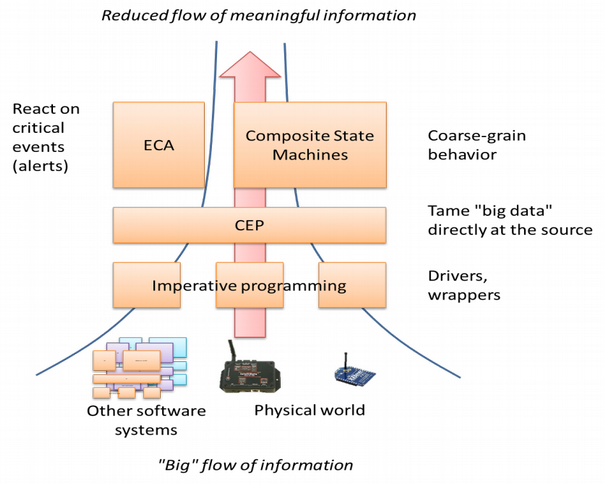
\includegraphics[width=0.7\linewidth]{figures/fig1}
\caption[Event Processing]{Event Processing}
\label{fig:fig1}
\end{figure}


As sensors might generate a large amount of data, a CEP layer close to the sensors enables service designers to express rules able to handle those data and to extract some relevant information (e.g. alert, status). The ECA paradigm is then particularly suited to handle alerts as they enable to enact some reflex-like actions (similarly to the way the spine "shortcuts" the brain to enact a fast movement e.g., when one burns his finger). Finally, composite state machines enable to describe advanced behavior, orchestrating and adapting to a set of events coming from the CEP. 

The HEADS Design Language is conceptually a usable sub-set of the UML (Composite Statecharts and Component Diagrams) with a syntactical notation rather than a graphical notation, so that it remains closer what programmers already know. In addition to the introduction of CEP in state machines, a key difference with UML is that our language comes with a first class action language so that models are not polluted with so-called "Opaque Behavior" (basically a String where code from the target language is directly outputted). This action language is basically the common subset of what is found in most languages, including numerical and Boolean algebra, control structures, functions, variable declaration and assignments, etc. The only action that is not typically found in programming language is the ability to asynchronously send a message through a port (rather than a simple method call). 

ECA rules are basically internal transitions, as in the JavaScript timer. Those rules basically react on an event and can be optionally guarded with any boolean expression, e.g. involving properties of the component and/or parameters of the message. Any action can then be triggered, either fully expressed at a platform-independent level or mixed with the target language (as in the JavaScript timer). As for the state machine, we support all the concepts present in the UML, including composite states and concurrent regions.  

The CEP concepts currently included in the HEADS Modeling Language is a sub-set of the concepts of ReactiveX (or other CEP language such a EPL available in Esper). We provide support for joining and merging flows of events, time or length windows and arbitrary filters.  

\begin{lstlisting}
stream lengthW 
  from e : [weather1?temp | weather2?temp]::keep if inRange(e)::during 1000*60 by 1000*60
  select avg : average(e.t[]),  
         min : min(e.t[]),  
         max : max(e.t[])  
action report!temp(avg, min, max)
\end{lstlisting}

This CEP stream illustrate most of the concepts currently integrated. It performs a merge between two temperature sensors (connected on ports weather1 and weather2). Basically, all temperature measurements coming from both sensor will be piped in a new stream. All these measurements are then filtered using a custom \texttt{inRange} operator defined by the developer, which will discard values that are outside a range and which are most likely due to an erroneous measurement rather than a correct measurement being too cold or too warn. The merging and the filtering happens on a time window during one minute which progress by slices of one minute. While such kind of CEP query could be implemented directly in Java, JavaScript or C, or at a more abstract level using the HEADS Modeling Language (state machine), it alleviates in any case the developer from writing a lot of "plumbing code" (timers, buffers, etc), which if not implemented correctly can have dramatic impact on memory and performances.

\subsection{HEADS Transformation Framework}

The HEADS Transformation Framework is responsible for ``compiling''  HEADS Design Models into source code for a large variety of languages. Rather than implementing one monolithic compiler for each language we target, the HEADS Transformation Framework instead is architected as a modular object-oriented framework. This framework promotes reuse of code among different compilers. A total of 8 formal extension points have been identified in the HEADS code generation framework in order to allow the developer to easily and efficiently customizing some parts of the code generation while reusing the rest. 

\subsubsection{Role of the extension points}

\paragraph{Actions / Expressions / Functions }


The implementation of this extension point consists of a visitor on the Actions and Expressions part of the HEADS Design Language. New code generators can be created by inheriting from that abstract visitor and implementing all its methods. Alternatively, if only a minor modification of an existing code generator is needed, it is possible to inherit from the existing visitor and only override a subset of its methods. Most of the actions and expressions (26 out of 35 concepts) is actually defined in the framework, as most of the programming languages have similar syntax for numerical and Boolean algebra, control structures, etc. The script below shows how a if  condition with optional else is compiled. The same code is reused in all Java, JavaScript and C compilers. 

\begin{lstlisting}[language=Java]
@Override 
public void generate(ConditionalAction action, StringBuilder builder, Context ctx) { 
  builder.append("if("); 
  generate(action.getCondition(), builder, ctx); 
  builder.append(") {\n"); 
  generate(action.getAction(), builder, ctx); 
  builder.append("\n}"); 
  if (action.getElseAction() != null) { 
    builder.append(" else {\n"); 
    generate(action.getElseAction(), builder, ctx); 
    builder.append("\n}"); 
  } 
  builder.append("\n"); 
} 
\end{lstlisting}

\paragraph{Behavior implementation}
This part of the code generator corresponds to the code generated from the state machine structures, ECA and CEP rules contained in Things. There is basically two main strategies to compile the behavior: target frameworks that are able to execute state machines and CEP or generate the whole logic to keep full control of what is executing at runtime. The first option is typically chosen for high-level languages not intended to run on resource-constrained devices, as it simplifies the code generation process (less code to generate) and generally improve the readability and maintainability of the generated code (less code to read and maintain). On resource-constrained devices however (down to 2 KB RAM) it is of primary importance to have control of every byte allocated and the overhead of embedding a framework is usually to heavy. The HEADS Transformation Framework does not impose nor favors any of those approaches and both can be implemented. The Java and JavaScript compilers use a framework approach whereas the family of C compilers use a full generative approach. In both cases, the framework provides support in the form of a set of helpers which pre-process the state machine e.g. to provide the list of all outgoing transitions for a given state, or the list of all messages being actually used by a component. 

\paragraph{Ports / Messages /APIs}

This part of the code generator corresponds to the wrapping of the generated code into reusable components on the target platform. Depending on the target platform, the language and the context in which the application is deployed, the code generated can be tailored to generate either custom modules or to fit particular coding constraints or middleware to be used on the target platform. As a best practice, the generated modules and APIs for things should be manually usable in case the rest of the system (or part of it) is written directly in the target language. For example, in object oriented languages, a facade and the observer pattern can be used to provide an easy to use API for the generated code. In C, a module with the proper header with structures and call-backs should be generated. 


The following code for example generates a Java interfaces that any Java programmer can use to send messages to a generated component. 

\begin{lstlisting}[language=Java]
for (Port p : thing.allPorts()) { 
  StringBuilder builder = ctx.getNewBuilder(thing.getName() + "_" + p.getName() + ".java"); 
  builder.append("public interface " + "I" +  
  thing.getName() + "_" + p.getName() + "{\n"); 
  for (Message m : p.getReceives()) { 
    builder.append("void " + m.getName() + "_via_" + p.getName() + "("); 
    generateParameter(m, builder, ctx); 
    builder.append(");\n"); 
  } 
  builder.append("}"); 
}
\end{lstlisting}

For example, for the Java timer component, this would generate this simple API: 


\begin{lstlisting}
public interface ITimerJava_timer{ 
	void start_via_timer(short delay); 
	void cancel_via_timer(); 
}
\end{lstlisting}

\paragraph{Main and Build}

These two extension points are responsible for providing users with a turn-key solution to compile and run the generated code. In the main file, all components and instantiated and connected. The build files automate all tasks needed to properly compile e.g. fetching dependency. For the users, compiling and running the code is as simple as: 

\begin{lstlisting}[language=bash]
mvn install exec:java #for Java 
npm install && node main.js #for JavaScript
make && ./myProgram #for C 
\end{lstlisting}

This extension point makes it easy to for example switch from Maven to Gradle for the build of Java project. 

\paragraph{Message Queing, Scheduling and Dispatching}

Those extension points are related to the internal management of messages within a node. By default, messages are queued in a FIFO, typically reusing already structures. On some very constrained platforms (microcontrollers) the code for the FIFO also needs to be generated as the standard library is typically more limited.For the scheduling and dispatching of messages we typically rely on facilities available on the OS (threads) to ensure a fair distribution of messages among components and avoid starvation and race conditions. Again, on very constrained platforms that are too limited to run an OS, custom schedulers should be generated.

\paragraph{Connectors}

This extension point is concerned with the serialization and transport of messages among components distributed over the network. For the serialization a default serialization of messages into arrays of bytes is provided~\cite{DBLP:conf/models/FleureyMSB11}, but developers can implement their own serialization. For example, we are currently implementing a generator to integrate with MessagePack~\cite{furuhashimessagepack}. For the transport itself, we usually rely on the large collections of communication channels already available in the HEADS Runtime platform (see next section): MQTT, WebSocket, Serial, etc. 

\subsubsection{Benefits of the HEADS Transformation Framework}
While the HEADS Transformation Framework can be seen as a family of compilers (producing code in Java, JavaScript and C/C++), those compilers have a different nature than a compiler like GCC, producing machine code out of C source code. Working at a higher level of abstraction, by transforming a model into source code rather than source code into machine code, drastically reduced the cost of writing a HEADS compiler. While GCC alone is about 14 millions LoC, the whole HEADS Transformation Framework, also including the compilers targeting Java, JavaScript and C/C++ is less than 25,000 LoC (560 times less). Those LoC are distributed (approx.) as follows:

\begin{itemize}
\item 6000 LoC in the framework itself, that all compilers reuse. This includes facilities to manage files, generate consistent variable names, etc. It also includes the code for compiling most of the actions and expressions (26 out of 35) of the HEADS Design Language. New compiler ({\em e.g.} targeting Go, Lua, PHP) will benefit from those 6000 LoC, unless the targeted language is radically different, for example if it uses a Polish notation like Lisp where "a + b" is expressed as "+ a b". 
\item 3000 LoC for the Java compiler that is able to generate fully working Java code. The generated code targets a framework for the execution of the state machines and another for the execution of CEP streams, hence most of the "tricky" code does not need to be generated as it is handled directly in those frameworks. In addition, 400 lines of code are needed to generate wrappers able to "merge" fine-grained implementation components into coarser-grained deployment components (as explained in the next sub-section) 
\item 3000 LoC for the JavaScript, which strictly follow the same approach as for the Java compiler. About 400 LoC are also needed to perform the wrapping. 
\item 11000 LoC for the family of C compilers, distributed (approx.) as follows: 
\begin{itemize}

\item 5000 for a generic C transformation framework shared by all C compilers 
\item 6000 LoC shared among a POSIX compiler for Linux, an AVR 8-bit compiler ({\em e.g.} for Arduino) and an ARM 32-bit compiler ({\em e.g.} for Cypress PSoC5).
\end{itemize}
\end{itemize}

Basically, supporting a new high-level language (like Java) with available libraries for state machines and CEP and having an infix (standard) notation should in most cases be limited to writing about 3000 LoC. Redifining the compilation of actions and expressions to support Polish (prefix) or postfix notation should be about 500 additional LoC. 
Supporting a lower-level language (like C) where libraries are not available (or do not provide enough control on the memory to be allocated, etc) is a slightly more complex endeavor, but still accessible to most programmers. Writing the POSIX C compiler for Linux was about 7000 LoC (as the code for execution of the state machine needs to be generated, etc), including the generic C transformation framework. However, supporting different ``dialects'' of C required about 2000 LoC for AVR 8-bit and 2000 LoC for ARM 32-bit, which is a limited effort. 


\subsection{HEADS Deployment Language and Runtime platform}

By default, the HEADS transformation framework generates standalone code that can be executed without any dependencies to HEADS tools and platforms. However, this code cannot easily be updated at runtime e.g. to substitute one component by another, though it is programmatically feasible to instantiate new components and connectors. In the HEADS Design language, components are indeed implementation units, in a way similar to Java classes. Wrapping each individual implementation unit in a deployable component having its own lifecycle at runtime would result in a large number of components that needs to be deployed and administrated at runtime. For example, in an implementation unit dealing with serial communication would typically be packed together with implementation units dealing with serialization/deserialization of messages in the same deploy unit. This way at runtime, the service operator would only need to deploy a single component responsible for serial communication, the (de)serialization aspect being hidden as an implementation detail. Figure \ref{fig:fig2} shows how HEADS implementation units can be wrapped into Heads deploy units.


\begin{figure}[t]
	\centering
	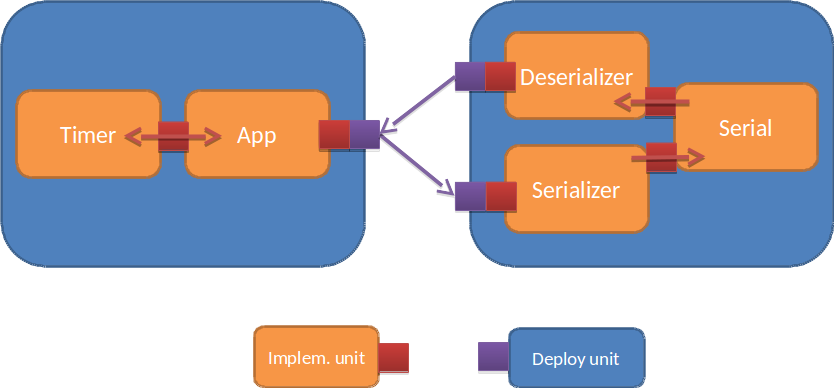
\includegraphics[width=0.8\linewidth]{figures/fig2}
	\caption[Heads implementation and deploy units integration]{Heads implementation and deploy units integration}
	\label{fig:fig2}
\end{figure}

Once wrapped into deploy units, components can be manipulated by the HEADS Deployment Language and actually deployed on the HEADS runtime platform, which evolves the Kevoree platform~\cite{DBLP:conf/cbse/FouquetMFBPJ12} initially developed for Java in order to also support JavaScript and more recently, .NET. The HEADS Deployment Language provide a way to write scripts describing which components to instantiate, how to configure them (set values of parameters), and how to connect components through communication channels. A large set of components and channels is already available off the shelf. At deployment time, the script, describing the components and channels deployed on the different nodes of the system, will be sent to the different nodes, which will interpret this script and actually deploy the necessary components, etc.   

The HEADS Deployment Language and Runtime platforms are available as a set of open-source projects on GitHub\footnote{https://github.com/dukeboard/kevoree\\https://github.com/kevoree/kevoree-js}.

\section{Enginering a Real-life eHealth Service with HEADS}

This section describes how the HEADS approach has been applied to the TellU's eHealth system. 

\subsection{Overall Architecture}
The overall architecture of the eHealth system is depicted in Figure~\ref{fig:fig3}. The system is composed of a home gateway which runs on a Raspberry Pi 2 (1 GHz ARMv7, 1GB RAM, Linux). This gateway is connected to a number of field nodes (typically one per main room in the house) via WiFi. Field nodes run on an Intel Edison (400 MHz x86, 1GB RAM, WiFi and Bluetooth Low Energy (BLE)). Each field node has a pressure cell integrated in order to provide an accurate measurement of the pressure in each room. A wearable sensor node running on a low power resource-constrained ARM Cortex M3 (80 MHz, 256 KB RAM) also integrates a pressure cell and regularly broadcasts air pressure measurement to all field node that are in the BLE range (typically 10m indoor). Based on these pressure measurements and the intensity of the BLE signal, field node can determine the position of the person in the house and if the person has feel (by computing an air pressure differential between the person's sensor and the fixed pressure in the field node). In addition, a set of sensor nodes are deployed in different rooms to measure temperature and light. Those nodes run on an Arduino Yùn, which is composed of a resource-constrained microcontroller (16 MHz AVR-8bit, 2.5 KB RAM, no OS) and an embedded Linux processor (400 MHz MIPS, 64 MB RAM, WiFi, OpenWRT). The microcontroller part of the Yùn is used to interact with the physical temperature and light sensors while the MIPS CPU and its embedded WiFi is used to communicate with the Gateway. Finally, the gateway also integrates a Z-Wave radio chip that can control and interact with a set of devices (switches, etc). 

\begin{figure*}[!t]
	\centering
	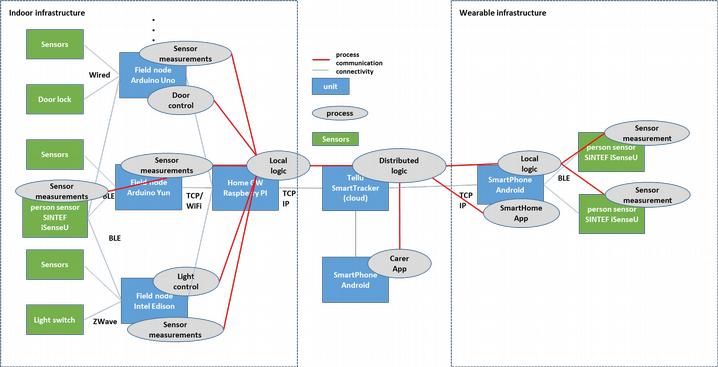
\includegraphics[width=0.8\linewidth]{figures/fig3}
	\caption{Safe@Home system architecture}
	\label{fig:fig3}
\end{figure*}



This particular HD-Service thus relies on an heterogeneous infrastructure composed from rather powerful 32-bit X86 and ARM processors with 1 GB RAM down to 8-bit AVR microcontroller running at 16 MHz (about 60 times slower) and embedding only 2.5 KB RAM (about 400 000 times less). It also integrates a variety of radio protocols such as WiFi, BlueTooth or Z-Wave. 

\subsection{Detailed Architecture and Implementation of the Field Node}

At design/implementation time, the Field Node is composed of 8 core components implementing the logic of the node, and 2 other components that allows the field node to push information to the gateway via MQTT. Each of the implementation component is available as: 
\begin{itemize}
\item A Platform-Independent Component (PIC), which describes the interfaces of the component i.e., the port and messages it exposes. Some PICs can also provide a full implementation of their behavior, if this behavior does not imply using low-level libraries/drivers that directly interfaces with the hardware or system APIs. 
\item A Platform-Specific Component (PSC), which describes the full behavior of a component including the access to hardware drivers and system APIs. 
\end{itemize}

For example, the PIC associated to the BLE component describes the following messages related to the status of the BLE connection: stateChange (st : String); discover (peripheral : String); scanStart (); scanStop (); startScanning (); stopScanning (); connect (peripheralId : String); disconnect (peripheralId : String); and discoverServices (peripheralId : String). Those messages are orchestrated in the BLE PSC by a state machine (see Figure \ref{fig:fig4}) interfacing with the "noble" JavaScript module to deal with low-level details related to BlueTooth. 

\begin{figure}[t]
	\centering
	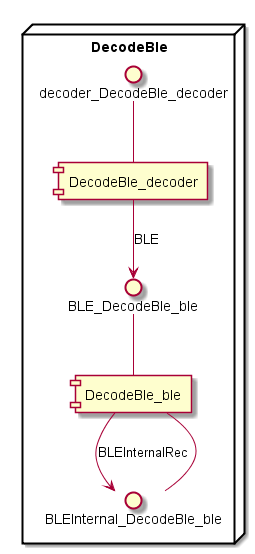
\includegraphics[width=0.5\linewidth]{figures/fig4}
	\caption{Component diagram of BLE and Decoder}
	\label{fig:fig4}
\end{figure}

Overall, the Field Node is implemented with ~300 LoC for the PICs and ~1100 LoC for the PSCs. It produces ~2000 LoC of JavaScript source code. This code can simply be run by executing the main.js file with Node.JS. However, this default implementation is rather monolithic at runtime and does not provide any dynamic reconfiguration capabilities. In order to provide such capabilities, this code is automatically wrapped into a component that can be manipulated and adapted at runtime. This additional component is fully generated and contained within 170 LoC. The automated wrapping is illustrated in Figure \ref{fig:fig5}. 

\begin{figure}[h]
	\centering
	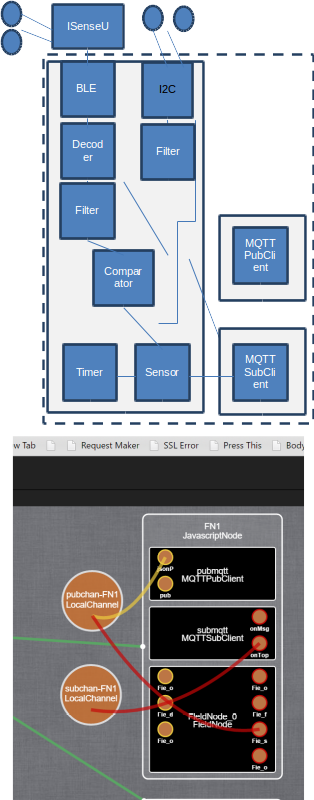
\includegraphics[width=0.6\linewidth]{figures/fig5}
	\caption{Field-Node component structure and EADS deployment of Field-Node seen in Heads deployment model editor}
	\label{fig:fig5}
\end{figure}


\subsection{Deployment and Operation of the Fall Detection service}
All the field node are described by 3 scripts. The first one is a root script basically describing the default configuration of the node, containing information about the network and how to connect to the rest of the system. It is shown in Figure~\ref{fig:fig6}

\begin{figure}[h]
	\centering
	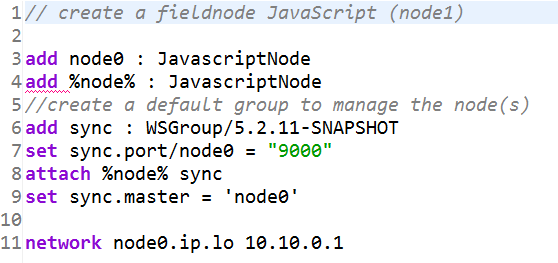
\includegraphics[width=0.7\linewidth]{figures/fig6}
	\caption{Default configuration of Field-Node}
	\label{fig:fig6}
\end{figure}

The second one is a script that will be executed whenever the field node connects to the network. This script adds a few components and connectors so that the field node can execute its logic and connect to the gateway via MQTT. This script is shown in Figure \ref{fig:fig7}. 
Finally, the third script simply remove the whole FieldNode from the model when the field node disappears from the network. Using those three scripts, the model and the running system are always in sync. Only field nodes that are actually connected to the network will appear in the model. For example Figure \ref{fig:fig8} shows the configuration of the running system after two field nodes have connected. 

\begin{figure}[h]
	\centering
	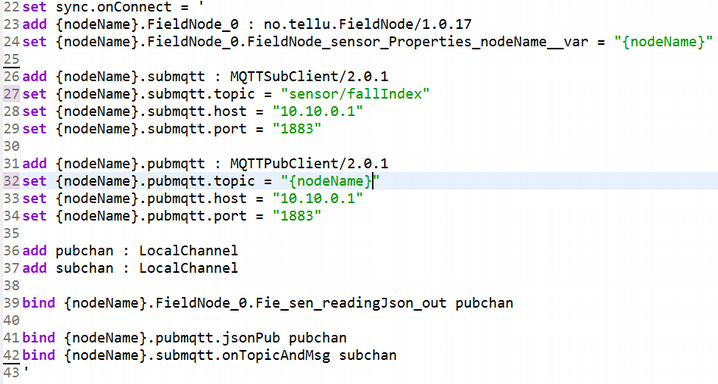
\includegraphics[width=1\linewidth]{figures/fig7}
	\caption{onConnect fragment of Home-GW inHEADS deployment model}
	\label{fig:fig7}
\end{figure}


\begin{figure}[h]
	\centering
	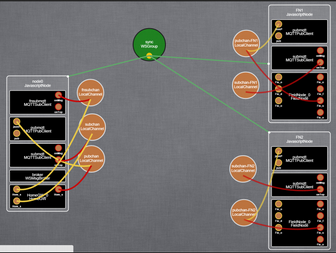
\includegraphics[width=1\linewidth]{figures/fig8}
	\caption{onConnect fragment of Home-GW inHEADS deployment model}
	\label{fig:fig8}
\end{figure}

\subsection{Summary}
The eHealth service implemented by the TellU company involves are rather heterogeneous infrastructure composed of X86, ARM, MIPS and AVR nodes, ranging from 1GHz CPU with 1GB RAM down to 16MHz microcontroller with 2.5 KB RAM. All the code generated for this service (in JavaScript for the larger nodes and C for the smaller nodes) worked out of the box, without any manual modifications. All the libraries TellU needed to use (to interact with Z-Wave, BlueTooth, GPIO on the Intel Edison, etc or to communicate over MQTT) could be integrated with no major issues, either in the HEADS Modelling Language, or directly in the target language as a HEADS component.  

A few limitations were noted by TellU. Deploying code on resource-constrained devices can sometimes be cumbersome, as the generated code first needs to be cross-compiled and then uploaded to the device. This limitation could easily be addressed by extending the extension point related to build scripts so that it could also run the scripts using a command line the user can override. By default the C compiler would just run make. When compiling and uploading to Arduino it would execute: avrdude -CD:avrdude.conf -v -v -v -v -patmega328p -carduino -P.COM22 -b57600 -D -Uflash:w:myProgram.cpp.hex:i 

Regarding the tooling, TellU was rather satisfied with the integration of the different languages and tools within the Eclipse IDE and simply noted some specific cases where code completion does not yet work on par with e.g. Java code completion. Other than that, the languages and tools are usable.

\subsection{Lessons learned}
Several developers at TellU, well acquainted with Java, were able to rapidly get started with the concepts and tools described in this approach. A series of tutorials covering the different concepts, and including exercises to be completed by the participants, was completed within a couple of days~\footnote{https://github.com/HEADS-project/training}. Before implementing the eHealth service, TellU developers have been working on the past few years on the backend service, collecting data and performing analytics. Integrating directly with sensors and gateways was thus a new activity. Most of the learning curve was related to learning how to interact directly with hardware. The HEADS approach actually speed up the process by allowing integrating with C and JavaScript libraries (not popular languages at TellU) without writing advanced C and JavaScript, as most of the logic could be expressed in a platform independent way. In particular, our generative and modular component-based approach for heterogeneous and distributed system allowed and efficient co-development and continuous evolution of this eHealth service. Once interfaces have been defined, it was easy for TellU to define mockups for the components that were not yet implemented and still be able to run the whole system. Mockups were replaced in an iterative way.

Regarding the integration with new languages and platforms, most of the compilers (POSIX C for Linux, Java and JavaScript) have been developed by people heavily involved in the definition of the HEADS Design Language and the Transformation Framework. It is thus hard to conclude on how difficult it is to implement a completely new compiler, other than it took 3000 LoC for Java and JavaScript and about 7000 LoC for POSIX C, which is far way less than writing a ``real'' compiler (GCC being 14 millions LoC). An experiment conducted with another department at SINTEF with people not involved in the development of the language and framework showed it is possible to extend the C compiler to support another ``dialect'' for ARM microcontrollers. This took about 2000 LoC and a couple of weeks for the embedded C expert (with only basic Java knowledge) to get this compiler fully functional. While the time to write this compiler could have been reduced e.g. with better documentation, the two weeks spend here were almost entirely saved by developers at TellU who could just get started with this new platform without building a detailed knowledge of C development on this platform.
%\input{validation}
\section{Related Work}

Some attempts of creating an "\textit{Esperanto2 of the programming languages}" have emerged, aiming at replacing the need for using multiple programming languages. For example, Haxe~\cite{dasnois2011haxe} is a programming language that cross-compile to most of the popular programming languages (Java, JavaScript, C++ and others). A significant development effort in Haxe, beyond the development of the language and compilers, is put in the development of a standard library (mostly wrapping the standard libraries of the targeted languages). This standard library needs to be embedded at runtime with a too large overhead to run on the most constrained platforms our approach is able to target. 

In the CBSE domain, some component platforms are available for different languages. For example, Fractal~\cite{bruneton2006fractal} is implemented in Java and C. However, no significant effort has been put to make the different platforms to interoperate 



\section{Conclusion}
%The conclusion goes here.





% conference papers do not normally have an appendix


% use section* for acknowledgment
\section*{Acknowledgment}

This work was funded by EU FP7/2007-2013 grant n611337, HEADS project (www.heads-project.eu)




% trigger a \newpage just before the given reference
% number - used to balance the columns on the last page
% adjust value as needed - may need to be readjusted if
% the document is modified later
%\IEEEtriggeratref{8}
% The "triggered" command can be changed if desired:
%\IEEEtriggercmd{\enlargethispage{-5in}}

% references section

% can use a bibliography generated by BibTeX as a .bbl file
% BibTeX documentation can be easily obtained at:
% http://mirror.ctan.org/biblio/bibtex/contrib/doc/
% The IEEEtran BibTeX style support page is at:
% http://www.michaelshell.org/tex/ieeetran/bibtex/
\bibliographystyle{IEEEtran}
% argument is your BibTeX string definitions and bibliography database(s)
\small
\bibliography{cbse}
%
% <OR> manually copy in the resultant .bbl file
% set second argument of \begin to the number of references
% (used to reserve space for the reference number labels box)
%\begin{thebibliography}{1}
	


%\end{thebibliography}




% that's all folks
\end{document}


